\begin{tabulka}[p]
\centering
\begin{tabular}{cc|cc|cc}
úhel (\si{\degree}) & intenzita & úhel (\si{\degree}) & intenzita & úhel (\si{\degree}) & intenzita \\ \hline
10,0 & 73 & 26,5 & 273 & 34,0 & 24 \\ 
12,0 & 56 & 27,0 & 1744 & 36,0 & 37 \\ 
14,0 & 67 & 27,5 & 2602 & 38,0 & 35 \\ 
16,0 & 50 & 28,0 & 2695 & 40,0 & 42 \\ 
18,0 & 46 & 28,5 & 2259 & 42,0 & 44 \\ 
20,0 & 51 & 29,0 & 1464 & 44,0 & 24 \\ 
22,0 & 46 & 29,5 & 866 & 46,0 & 39 \\ 
24,0 & 55 & 30,0 & 462 & 48,0 & 35 \\ 
26,0 & 88 & 32,0 & 42 & 50,0 & 36 \\
\end{tabular}
\caption{Úhlová závislost intenzity při pevné orientaci krystalu $\vartheta=\SI{14}{\degree}$}
\label{t:uhel}
\end{tabulka}


\begin{tabulka}[p]
\centering
\begin{tabular}{ccc|ccc}
$\vartheta$ (\si{\degree}) & $\lambda$ (\si{\pico\metre}) & $I$ & $\vartheta$ (\si{\degree}) & $\lambda$ (\si{\pico\metre}) & $I$   \\ \hline
5,0 & 35 & 90 & 18,0 & 125 & 1247 \\ 
5,5 & 39 & 96 & 18,5 & 128 & 1117 \\ 
6,0 & 42 & 73 & 19,0 & 132 & 1227 \\ 
6,5 & 46 & 55 & 19,5 & 135 & 1193 \\ 
7,0 & 49 & 76 & 20,0 & 138 & 1094 \\ 
7,5 & 53 & 58 & 20,5 & 142 & 2008 \\ 
8,0 & 56 & 68 & \underline{21,0} & \underline{145} & \underline{6050} \\ 
\textbf{8,5} & \textbf{60} & \textbf{62} & 21,5 & 148 & 1196 \\ 
9,0 & 63 & 334 & 22,0 & 152 & 908 \\ 
9,5 & 67 & 1150 & 22,5 & 155 & 1132 \\ 
10,0 & 70 & 1673 & \underline{23,0} & \underline{158} & \underline{18646} \\ 
10,5 & 74 & 2159 & 23,5 & 161 & 11208 \\ 
11,0 & 77 & 2526 & 24,0 & 165 & 631 \\ 
11,5 & 81 & 2590 & 24,5 & 168 & 490 \\ 
12,0 & 84 & 2706 & 25,0 & 171 & 453 \\ 
12,5 & 88 & 2669 & 25,5 & 174 & 431 \\ 
13,0 & 91 & 2663 & 26,0 & 177 & 326 \\ 
13,5 & 94 & 2588 & 26,5 & 181 & 334 \\ 
14,0 & 98 & 2554 & 27,0 & 184 & 304 \\ 
14,5 & 101 & 2137 & 27,5 & 187 & 323 \\ 
15,0 & 105 & 1954 & 28,0 & 190 & 246 \\ 
15,5 & 108 & 1654 & 28,5 & 193 & 238 \\ 
16,0 & 112 & 1613 & 29,0 & 196 & 234 \\ 
16,5 & 115 & 1506 & 29,5 & 199 & 210 \\ 
17,0 & 118 & 1544 & 30,0 & 202 & 181 \\ 
17,5 & 122 & 1312 &  &  &  \\ 
\end{tabular}
\caption{Spektrum rentgenového záření při konstantním anodovém napětí rentgenky $U_a=\SI{21}{\kV}$}
\label{t:spektrum}
\end{tabulka}


\begin{tabulka}[p]
\centering
\begin{tabular}{ccc|ccc}
\multicolumn{3}{c|}{$U_a = \SI{20}{\kV}$} & \multicolumn{3}{c}{$U_a = \SI{18}{\kV}$} \\
$\vartheta$ (\si{\degree}) & $\lambda$ (\si{\pico\metre}) & $I$ & $\vartheta$ (\si{\degree}) & $\lambda$ (\si{\pico\metre}) & $I$   \\ \hline
8,5 & 60 & 56 & 9,5 & 67 & 40 \\ 
\textbf{9,0} & \textbf{63} & \textbf{45} & \textbf{10,0} & \textbf{70} & \textbf{77} \\ 
9,5 & 67 & 277 & 10,5 & 74 & 362 \\ 
10,0 & 70 & \textgreater 800 &  &  &  \\ 
\end{tabular}
\caption{Spektrum v okolí mezní vlnové délky pro různá anodová napětí}
\label{t:mezni}
\end{tabulka}


\begin{graph}[p] 
\centering
% GNUPLOT: LaTeX picture with Postscript
\begingroup
  \makeatletter
  \providecommand\color[2][]{%
    \GenericError{(gnuplot) \space\space\space\@spaces}{%
      Package color not loaded in conjunction with
      terminal option `colourtext'%
    }{See the gnuplot documentation for explanation.%
    }{Either use 'blacktext' in gnuplot or load the package
      color.sty in LaTeX.}%
    \renewcommand\color[2][]{}%
  }%
  \providecommand\includegraphics[2][]{%
    \GenericError{(gnuplot) \space\space\space\@spaces}{%
      Package graphicx or graphics not loaded%
    }{See the gnuplot documentation for explanation.%
    }{The gnuplot epslatex terminal needs graphicx.sty or graphics.sty.}%
    \renewcommand\includegraphics[2][]{}%
  }%
  \providecommand\rotatebox[2]{#2}%
  \@ifundefined{ifGPcolor}{%
    \newif\ifGPcolor
    \GPcolorfalse
  }{}%
  \@ifundefined{ifGPblacktext}{%
    \newif\ifGPblacktext
    \GPblacktexttrue
  }{}%
  % define a \g@addto@macro without @ in the name:
  \let\gplgaddtomacro\g@addto@macro
  % define empty templates for all commands taking text:
  \gdef\gplbacktext{}%
  \gdef\gplfronttext{}%
  \makeatother
  \ifGPblacktext
    % no textcolor at all
    \def\colorrgb#1{}%
    \def\colorgray#1{}%
  \else
    % gray or color?
    \ifGPcolor
      \def\colorrgb#1{\color[rgb]{#1}}%
      \def\colorgray#1{\color[gray]{#1}}%
      \expandafter\def\csname LTw\endcsname{\color{white}}%
      \expandafter\def\csname LTb\endcsname{\color{black}}%
      \expandafter\def\csname LTa\endcsname{\color{black}}%
      \expandafter\def\csname LT0\endcsname{\color[rgb]{1,0,0}}%
      \expandafter\def\csname LT1\endcsname{\color[rgb]{0,1,0}}%
      \expandafter\def\csname LT2\endcsname{\color[rgb]{0,0,1}}%
      \expandafter\def\csname LT3\endcsname{\color[rgb]{1,0,1}}%
      \expandafter\def\csname LT4\endcsname{\color[rgb]{0,1,1}}%
      \expandafter\def\csname LT5\endcsname{\color[rgb]{1,1,0}}%
      \expandafter\def\csname LT6\endcsname{\color[rgb]{0,0,0}}%
      \expandafter\def\csname LT7\endcsname{\color[rgb]{1,0.3,0}}%
      \expandafter\def\csname LT8\endcsname{\color[rgb]{0.5,0.5,0.5}}%
    \else
      % gray
      \def\colorrgb#1{\color{black}}%
      \def\colorgray#1{\color[gray]{#1}}%
      \expandafter\def\csname LTw\endcsname{\color{white}}%
      \expandafter\def\csname LTb\endcsname{\color{black}}%
      \expandafter\def\csname LTa\endcsname{\color{black}}%
      \expandafter\def\csname LT0\endcsname{\color{black}}%
      \expandafter\def\csname LT1\endcsname{\color{black}}%
      \expandafter\def\csname LT2\endcsname{\color{black}}%
      \expandafter\def\csname LT3\endcsname{\color{black}}%
      \expandafter\def\csname LT4\endcsname{\color{black}}%
      \expandafter\def\csname LT5\endcsname{\color{black}}%
      \expandafter\def\csname LT6\endcsname{\color{black}}%
      \expandafter\def\csname LT7\endcsname{\color{black}}%
      \expandafter\def\csname LT8\endcsname{\color{black}}%
    \fi
  \fi
  \setlength{\unitlength}{0.0500bp}%
  \begin{picture}(10204.00,4534.00)%
    \gplgaddtomacro\gplbacktext{%
      \csname LTb\endcsname%
      \put(396,484){\makebox(0,0){\strut{} 10}}%
      \csname LTb\endcsname%
      \put(1572,484){\makebox(0,0){\strut{} 15}}%
      \csname LTb\endcsname%
      \put(2749,484){\makebox(0,0){\strut{} 20}}%
      \csname LTb\endcsname%
      \put(3925,484){\makebox(0,0){\strut{} 25}}%
      \csname LTb\endcsname%
      \put(5102,484){\makebox(0,0){\strut{} 30}}%
      \csname LTb\endcsname%
      \put(6278,484){\makebox(0,0){\strut{} 35}}%
      \csname LTb\endcsname%
      \put(7454,484){\makebox(0,0){\strut{} 40}}%
      \csname LTb\endcsname%
      \put(8631,484){\makebox(0,0){\strut{} 45}}%
      \csname LTb\endcsname%
      \put(9807,484){\makebox(0,0){\strut{} 50}}%
      \put(176,2486){\rotatebox{-270}{\makebox(0,0){\strut{}intenzita}}}%
      \put(5101,154){\makebox(0,0){\strut{}úhel (\si{\degree})}}%
    }%
    \gplgaddtomacro\gplfronttext{%
    }%
    \gplbacktext
    \put(0,0){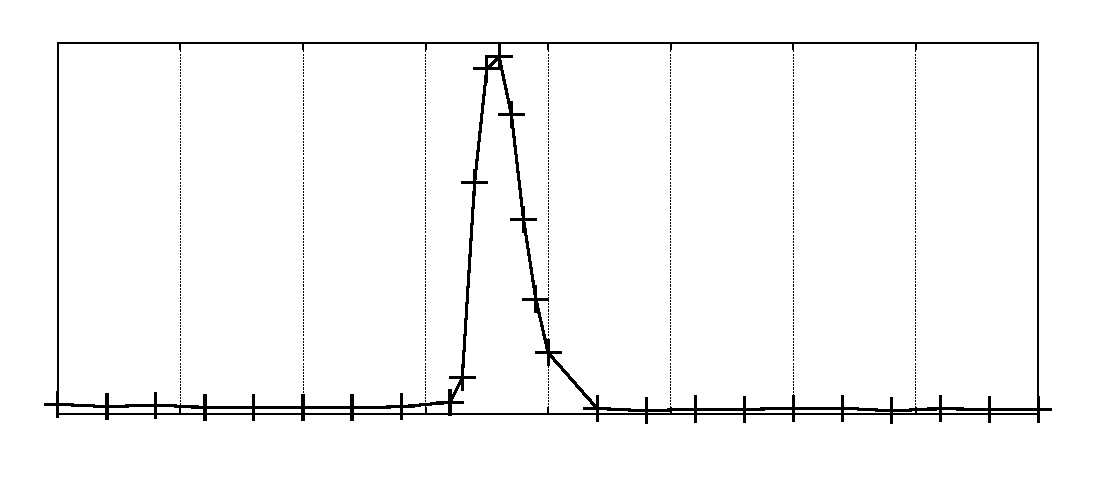
\includegraphics{uhel}}%
    \gplfronttext
  \end{picture}%
\endgroup

\caption{Úhlová závislost intenzity při pevné orientaci krystalu $\vartheta=\SI{14}{\degree}$}
\label{g:uhel}
\end{graph}


\begin{graph}[p] 
\centering
% GNUPLOT: LaTeX picture with Postscript
\begingroup
  \makeatletter
  \providecommand\color[2][]{%
    \GenericError{(gnuplot) \space\space\space\@spaces}{%
      Package color not loaded in conjunction with
      terminal option `colourtext'%
    }{See the gnuplot documentation for explanation.%
    }{Either use 'blacktext' in gnuplot or load the package
      color.sty in LaTeX.}%
    \renewcommand\color[2][]{}%
  }%
  \providecommand\includegraphics[2][]{%
    \GenericError{(gnuplot) \space\space\space\@spaces}{%
      Package graphicx or graphics not loaded%
    }{See the gnuplot documentation for explanation.%
    }{The gnuplot epslatex terminal needs graphicx.sty or graphics.sty.}%
    \renewcommand\includegraphics[2][]{}%
  }%
  \providecommand\rotatebox[2]{#2}%
  \@ifundefined{ifGPcolor}{%
    \newif\ifGPcolor
    \GPcolorfalse
  }{}%
  \@ifundefined{ifGPblacktext}{%
    \newif\ifGPblacktext
    \GPblacktexttrue
  }{}%
  % define a \g@addto@macro without @ in the name:
  \let\gplgaddtomacro\g@addto@macro
  % define empty templates for all commands taking text:
  \gdef\gplbacktext{}%
  \gdef\gplfronttext{}%
  \makeatother
  \ifGPblacktext
    % no textcolor at all
    \def\colorrgb#1{}%
    \def\colorgray#1{}%
  \else
    % gray or color?
    \ifGPcolor
      \def\colorrgb#1{\color[rgb]{#1}}%
      \def\colorgray#1{\color[gray]{#1}}%
      \expandafter\def\csname LTw\endcsname{\color{white}}%
      \expandafter\def\csname LTb\endcsname{\color{black}}%
      \expandafter\def\csname LTa\endcsname{\color{black}}%
      \expandafter\def\csname LT0\endcsname{\color[rgb]{1,0,0}}%
      \expandafter\def\csname LT1\endcsname{\color[rgb]{0,1,0}}%
      \expandafter\def\csname LT2\endcsname{\color[rgb]{0,0,1}}%
      \expandafter\def\csname LT3\endcsname{\color[rgb]{1,0,1}}%
      \expandafter\def\csname LT4\endcsname{\color[rgb]{0,1,1}}%
      \expandafter\def\csname LT5\endcsname{\color[rgb]{1,1,0}}%
      \expandafter\def\csname LT6\endcsname{\color[rgb]{0,0,0}}%
      \expandafter\def\csname LT7\endcsname{\color[rgb]{1,0.3,0}}%
      \expandafter\def\csname LT8\endcsname{\color[rgb]{0.5,0.5,0.5}}%
    \else
      % gray
      \def\colorrgb#1{\color{black}}%
      \def\colorgray#1{\color[gray]{#1}}%
      \expandafter\def\csname LTw\endcsname{\color{white}}%
      \expandafter\def\csname LTb\endcsname{\color{black}}%
      \expandafter\def\csname LTa\endcsname{\color{black}}%
      \expandafter\def\csname LT0\endcsname{\color{black}}%
      \expandafter\def\csname LT1\endcsname{\color{black}}%
      \expandafter\def\csname LT2\endcsname{\color{black}}%
      \expandafter\def\csname LT3\endcsname{\color{black}}%
      \expandafter\def\csname LT4\endcsname{\color{black}}%
      \expandafter\def\csname LT5\endcsname{\color{black}}%
      \expandafter\def\csname LT6\endcsname{\color{black}}%
      \expandafter\def\csname LT7\endcsname{\color{black}}%
      \expandafter\def\csname LT8\endcsname{\color{black}}%
    \fi
  \fi
  \setlength{\unitlength}{0.0500bp}%
  \begin{picture}(10204.00,6802.00)%
    \gplgaddtomacro\gplbacktext{%
      \csname LTb\endcsname%
      \put(396,484){\makebox(0,0){\strut{} 0}}%
      \csname LTb\endcsname%
      \put(844,484){\makebox(0,0){\strut{} 10}}%
      \csname LTb\endcsname%
      \put(1292,484){\makebox(0,0){\strut{} 20}}%
      \csname LTb\endcsname%
      \put(1740,484){\makebox(0,0){\strut{} 30}}%
      \csname LTb\endcsname%
      \put(2189,484){\makebox(0,0){\strut{} 40}}%
      \csname LTb\endcsname%
      \put(2637,484){\makebox(0,0){\strut{} 50}}%
      \csname LTb\endcsname%
      \put(3085,484){\makebox(0,0){\strut{} 60}}%
      \csname LTb\endcsname%
      \put(3533,484){\makebox(0,0){\strut{} 70}}%
      \csname LTb\endcsname%
      \put(3981,484){\makebox(0,0){\strut{} 80}}%
      \csname LTb\endcsname%
      \put(4429,484){\makebox(0,0){\strut{} 90}}%
      \csname LTb\endcsname%
      \put(4877,484){\makebox(0,0){\strut{} 100}}%
      \csname LTb\endcsname%
      \put(5326,484){\makebox(0,0){\strut{} 110}}%
      \csname LTb\endcsname%
      \put(5774,484){\makebox(0,0){\strut{} 120}}%
      \csname LTb\endcsname%
      \put(6222,484){\makebox(0,0){\strut{} 130}}%
      \csname LTb\endcsname%
      \put(6670,484){\makebox(0,0){\strut{} 140}}%
      \csname LTb\endcsname%
      \put(7118,484){\makebox(0,0){\strut{} 150}}%
      \csname LTb\endcsname%
      \put(7566,484){\makebox(0,0){\strut{} 160}}%
      \csname LTb\endcsname%
      \put(8014,484){\makebox(0,0){\strut{} 170}}%
      \csname LTb\endcsname%
      \put(8463,484){\makebox(0,0){\strut{} 180}}%
      \csname LTb\endcsname%
      \put(8911,484){\makebox(0,0){\strut{} 190}}%
      \csname LTb\endcsname%
      \put(9359,484){\makebox(0,0){\strut{} 200}}%
      \csname LTb\endcsname%
      \put(9807,484){\makebox(0,0){\strut{} 210}}%
      \put(176,3620){\rotatebox{-270}{\makebox(0,0){\strut{}$I$}}}%
      \put(5101,154){\makebox(0,0){\strut{}$\lambda$ (\si{\pico\metre})}}%
    }%
    \gplgaddtomacro\gplfronttext{%
    }%
    \gplbacktext
    \put(0,0){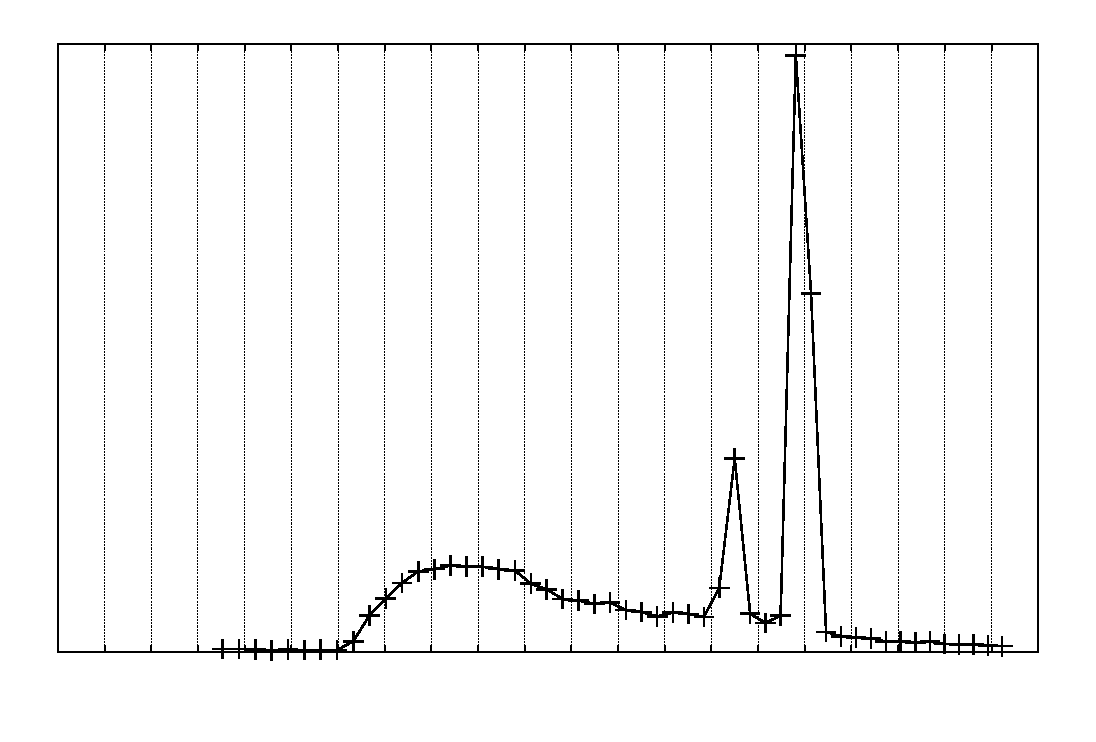
\includegraphics{spektrum}}%
    \gplfronttext
  \end{picture}%
\endgroup

\caption{Spektrum rentgenového záření při konstantním anodovém napětí rentgenky $U_a=\SI{21}{\kV}$}
\label{g:spektrum}
\end{graph}